\Chapter{CONTEXTE ET TRAVAUX CONNEXES}\label{chap:revue}

% Text

On présente ici le contexte général de nos travaux, ainsi qu'un aperçu de la littérature existante.
La section \ref{sec:dl} introduit les concepts fondamentaux du Web sémantique : les graphes de connaissance, qui offrent une représentation structurée de la connaissance, et la logique descriptive, qui permet d'enrichir ces graphes de règles logiques dont la somme constitue une taxonomie ou une ontologie, selon les cas.

Nous présentons ensuite les techniques existantes pour extraire automatiquement des taxonomies ou des ontologies. Cette tâche d'extraction automatique a en effet fait l'objet de nombreux travaux : nous résumons ici les principales approches ainsi que les idées notables du domaine, en distinguant notamment les approches basées sur du texte, que l'on présente à la section \ref{subsec:litt-te-text}, et les approches basées sur les graphes, qui sont décrites dans la section \ref{subsec:litt-te-graph}.

Notons enfin que les plongements vectoriels de graphe, qui constituent le socle de notre travail, font l'objet d'un chapitre dédié (chapitre \ref{chap:kge}).


\section{Web sémantique et logique descriptive}
\label{sec:dl}

\subsection{Graphes de connaissance}

% À déplacer vers l'INtroduction ??

%Un graphe de connaissance permet de représenter des données de manière structurée. Il consiste en un ensemble d'objets du monde réel, appellés \textit{entités}, reliés entre eux par des \textit{relations}.

%On se donne $\Ent$ un ensemble d'entités, et $\Rel$ un ensemble de relations. En pratique, chaque entité ou relation est représentée par un identifiant unique, l'IRI (\textit{Universal Resource Identifier}).

%Un graphe de connaissance 

Un graphe de connaissance est une collection structurée de données permettant de représenter des informations, ou des \textit{faits}, sur le monde réel. La définition exacte d'un graphe de connaissance varie d'un auteur à l'autre \cite{ehrlinger2016towards}; parmi les caractéristiques fréquemment retenues, on notera l'interconnexion des données et le caractère multi-relationnel, l'existence d'une sémantique formelle et de mécanismes de raisonnement, et parfois une certaine taille critique. Les paragraphes suivants visent à définir et expliciter ces différentes propriétés.


\paragraph{Concepts de base}

Dans ce travail, on adopte une définition très générale d'un graphe de connaissance vu comme un ensemble d'\textit{entités} liées entre elles par des \textit{relations}. Pour un ensemble d'entités $\Ent$ et un ensemble de relations $\Rel$, un graphe de connaissance est simplement un ensemble de triplets $\KG \subseteq \Ent \times \Rel \times \Ent$. Si $(h, r, t)$ est un triplet du graphe, alors l'entité $h$ est reliée à l'entité $t$ par la relation $r$; dans ce cas, on dit que $h$ est le \textit{sujet} du triplet, et $t$ son objet. Le choix des notations s'explique par l'anglais, $h$ désignant la tête (\textit{head}) et $t$ la queue (\textit{tail}) du triplet. Dans la suite, on désignera par \textit{voisinage} d'une entité l'ensemble des triplets qui impliquent cette entité en tant que sujet ou objet, et on notera $\rel{h}{r}{t}$ pour indiquer que le triplet $(h, r, t)$ est présent dans le graphe.
% Pour un graphe de connaissance, on parle fréquement de données \textit{multi-relationnelles} pour indiquer que les entités

En pratique, lorsqu'on parle de graphe de connaissance, on s'attend à quelques restrictions supplémentaires. D'une part, les données d'un graphe de connaissance doivent être \textit{multi-relationnelles}, c'est-à-dire qu'il doit exister plusieurs relations possibles entre les entités ($| \Rel | > 1$); d'autre part, les entités sont reliées \textit{mutuellement} entre elles. Ainsi, un système reliant des fichiers à des méta-données textuelles ne saurait être qualifié de graphe de connaissance; dans un graphe de connaissance, les objets d'un triplet sont, au moins pour partie, sujets d'autre triplets, et le graphe forme donc un réseau d'entités interconnectées. 


Le format dominant pour représenter un tel graphe est le format RDF, pour \textit{Resource Description Framework} \cite{cyganiak14}. En RDF, les éléments sont de deux types : soit des identifiants, soit des littéraux. Les \textbf{identifants}, ou IRI, pour \textit{International Resource Identifier}, sont simplement des chaînes de caractères qui désignent des ressources du monde réel : lieux, personnes, documents, etc. Les IRI servent également à représenter les relations du graphe.
RDF n'impose pas de mécanisme pour relier les IRI aux entités qu'elles désignent : c'est au créateur du graphe d'établir cette correspondance. Dans le cadre du Web des données, les IRI prennent la forme d'un lien HTTP.
Les \textbf{littéraux} permettent de représenter des valeurs fixes : nombres, textes, booléens, dates, sommes d'argent. Contrairement aux identifiants, l'interprétation des littéraux est définie une fois pour toutes; la manière d'interpréter un littéral est indiquée par son \textit{format} (parfois appelé \textit{datatype} en anglais). Par exemple, le littéral \texttt{1901-01-28\^{}\^{}xsd:date} est constitué de la valeur \texttt{1901-01-28} au format \texttt{xsd:date}, et s'interprète de manière unique comme la date du 28 janvier 1901.

Un \textit{vocabulaire} est un ensemble d'IRI, présentant une certaine cohérence. Les IRI d'un même vocabulaire partagent quasi-systématiquement une racine commune, que l'on peut alors abréger par un \textit{préfixe}. Ainsi, toutes les IRI du vocabulaire standard RDF commencent par \texttt{http://www.w3.org/1999/02/22-rdf-syntax-ns\#}, que l'on abrège en \texttt{rdf:}. Par exemple, les IRI \texttt{http://www.w3.org/1999/02/22-rdf-syntax-ns\#type} et \texttt{http://www.w3.org/199-9/02/22-rdf-syntax-ns\#Property} sont abrégées en \texttt{rdf:type} et \texttt{rdf:Property}, respectivement. 


% De la même manière, les entités de DBpedia sont regroupées dans un vocabulaire commun, dont le préfixe usuel est \texttt{dbr} (abrégé de \texttt{http://dbpedia.org/resource/}) : ainsi, \dbr{Montréal} ou \dbr{Pablo\_Picasso} désignent des entités de DBpedia.

% DBpedia

\paragraph{Un exemple : DBpedia}

Il existe de nombreux graphes de connaissance publics; certains sont restreints à un domaine spécifique, comme UniProt \cite{uniprot2017uniprot} ou DrugBank \cite{wishart2018drugbank}, % WordNet \cite{miller1998wordnet},
d'autres sont généralistes, comme YAGO \cite{suchanek2008yago} ou Wikidata \cite{vrandevcic2014wikidata}. Parmi ces graphes de connaissances généralistes, l'un des plus notables est DBpedia \cite{auer2007dbpedia}, sur lequel on s'appuiera dans toute la suite de ce travail, dans sa version anglaise. Les données de DBpedia sont obtenues de manière automatique en agrégeant différentes sources structurées ou semi-structurées issues de Wikipédia. Le cœur de DBpedia est son système d'extraction, qui convertit Wikipédia en un ensemble de triplets RDF à l'aide de différentes heuristiques; cet extracteur s'appuie essentiellement sur les infoboîtes de Wikipédia, des encarts constituées de paires clé-valeur et dont le format est relativement uniformisé à l'échelle de Wikipédia. Outre les infoboîtes, l'extracteur utilise également les liens de redirection et de désambiguïsation, les catégories des pages, les éventuelles informations de géolocalisation, etc. À cet extracteur s'ajoutent différentes procédures pour nettoyer et uniformiser les résultats, ainsi que pour agréger des données provenant d'autres sources. DBpedia fournit également un point d'entrée pour effectuer des requêtes sur le graphe\footnote{\href{https://dbpedia.org/sparql}{dbpedia.org/sparql}}.

Les entités de DBpedia sont regroupées au sein d'un vocabulaire \texttt{http://dbpedia.org/resource/}, généralement abrégé en \dbr{}. Le voisinage d'une entité donnée \dbr{<Nom de l'entité>} %, c'est-à-dire les triplets dont cette entité est le sujet ou l'objet, 
peut être consulté en ligne à l'adresse \href{http://dbpedia.org/page/<Nom de l'entité>}{dbpedia.org/page/<Nom de l'entité>}. Les relations et les classes de DBpedia font elles parties du vocabulaire \texttt{http://dbpedia.org/ontology/}, abrégé en \dbo{}. DBpedia fait parfois appel à des relations ou des classes issues d'autres vocabulaires, dont FOAF\footnote{\href{http://xmlns.com/foaf/spec/}{xmlns.com/foaf/spec/}} et Dublin Core\footnote{\href{https://dublincore.org/}{dublincore.org/}}.


DBpedia contient à l'heure actuelle 1 300 relations et 4,2 millions d'entités pour un total de 56,5 millions de triplets. Les entités sont réparties selon 655 types, dont les plus fréquents sont les personnes (\dbo{Person}), les lieux (\dbo{Place}), les espèces (\dbo{Species}), les événements (\dbo{Event}), les œuvres (\dbo{Work}), les organisations (\dbo{Organisation}). Comme les données de DBpedia sont extraites automatiquement de Wikipédia et que Wikipédia est modifié régulièrement, le graphe DBpedia évolue lui aussi régulièrement.


\paragraph{Typologie des relations} 

Il est utile de détailler les propriétés que peuvent avoir les relations dans un graphe de connaissance, et en premier lieu leur caractère symétrique ou antisymétrique :
Nous citons ici les deux propriétés qui serviront dans la suite du mémoire, à savoir la transitivité et la symétrie :
\begin{itemize}
    \item une relation $r$ est \textbf{transitive} si l'existence des liens $\rel{x}{r}{y}$ et $\rel{y}{r}{z}$ implique l'existence de $\rel{x}{r}{z}$ : c'est le cas notamment des relation \dbo{ancestor} et \dbo{isPartOf};
    \item une relation $r$ est \textbf{symétrique} si $\rel{t}{r}{h}$ est vérifiée dès que $\rel{h}{r}{t}$ est vérifiée. Par exemple, la relation \texttt{owl:sameAs}, qui indique que deux IRI correspondent à la même entité, est naturellement symétrique. Plus généralement, toutes les relations qui impliquent une équivalence ou une réciprocité sont symétriques, comme \dbo{spouse} ou \dbo{colleague};
    \item à l'inverse, une relation $r$ est \textbf{antisymétrique} si $\rel{h}{r}{t}$ et $\rel{t}{r}{h}$ ne peuvent jamais être vérifiées simultanément. C'est le cas, en pratique, de la plupart des relations hiérarchiques comme \texttt{rdfs:subClassOf} ou \dbo{parent};
\end{itemize}
Une relation peut très bien n'être ni symétrique, ni antisymétrique. La relation \dbo{influenced}, qui marque l'influence intellectuelle d'une personne sur un autre, est parfois mutuelle (pensons par exemple à Russell et Wittgenstein, ou Beauvoir et Sartre) et parfois non.


% Une relation est dite \textit{réflexive} si une entité est toujours reliée à elle-même par cette relation, et \textit{irréflexive} si une entité ne peut pas être reliée à elle-même. Par exemple, les relations d'inclusion \texttt{isPartOf} et d'inclusion stricte \texttt{isProperPartOf} entre des ensembles sont respectivement réflexive et irréflexive. Enfin, une relation $r$ est \textit{transitive} si l'existence des liens $\rel{x}{r}{y}$ et $\rel{y}{r}{z}$ implique l'existence de $\rel{x}{r}{z}$ : c'est le cas notamment de la relation \dbo{ancestor}

On peut également classer les relations selon les cardinalités relatives de leurs sujets et de leurs objets :
\begin{itemize}
    \item une relation \textbf{\textit{one-to-many}} (de un à plusieurs, en français) lie chaque sujet à plusieurs objets : par exemple, pour la relation \dbo{product}, 
    une marque est reliée à tous les produits qu'elle commercialise, tandis qu'un produit ne possède qu'une seule marque;
    \item à l'opposé, une relation \textbf{\textit{many-to-one}} (de plusieurs à un) lie plusieurs sujets à un même objet; c'est le cas de la relation \texttt{foaf:gender} qui, dans DBpedia, relie un million et demi de sujets à seulement trois objets (\texttt{"male"}, \texttt{"female"} et \texttt{"non-binary"});
    \item une relation \textbf{\textit{one-to-one}} (un pour un) relie un sujet à un unique objet, et réciproquement. On peut penser à la relation qui unit un pays à sa capitale (\dbo{capital}), ou une entité à son label (\texttt{rdfs:label});
    \item enfin, une relation \textbf{\textit{many-to-many}} (de plusieurs à plusieurs) relie un sujet à plusieurs objets, et un objet à plusieurs sujets. Cette catégorie comprend par exemple la relation \dbo{influencedBy} citée plus haut : en général, un artiste ou un penseur est influencé par plusieurs personnes, et en influence d'autres à son tour;
\end{itemize}

%En parallèle de cette classification stricte des relations, il est parfois intéressant de comparer le
Pour déterminer à quelle catégorie appartient une relation, il suffit de comparer le nombre moyen d'objets par sujet au nombre moyen de sujets par objet \cite{transh}. Pour une relation $r$ donnée, on note $tph_r$ (de l'anglais \textit{tails per head}) le nombre moyen d'objets reliés à une entité par la relation $r$ :
\begin{equation}
    tph_r = \frac{\sum_{h \in \Ent} |\{ t \in \Ent : \rel{h}{r}{t} \}|}{|\{ h \in \Ent : \exists y \in \Ent, \rel{h}{r}{y} \}| }
\end{equation}
Et, réciproquement, on note $hpt_r$ (de l'anglais \textit{heads per tail}) le nombre moyen de sujets qui sont relié à un objet par la relation $r$. 

Dès lors, une relation $r$ est \textit{one-to-many} si $hpt_r = 1$ et $tph_r > 1$, \textit{many-to-one} si $hpt_r > 1$ et $tph_r = 1$, \textit{one-to-one} si $hpt_r = tph_r = 1$, et \textit{many-to-many} si $hpt_r > 1$ et $tph_r > 1$. En pratique, pour les graphes de connaissance extraits automatiquement, cette classification est très stricte; certains auteurs comme \cite{bordes2013translating, transh} proposent de tenir compte du bruit des données en caractérisant les relations \textit{one-to-many} par $hpt_r \leq 1,5$ et $tph_r > 1,5$, \textit{many-to-one} par $hpt_r > 1,5$ et $tph_r \leq 1,5$, \textit{one-to-one} par $hpt_r \leq 1,5$ et $tph_r \leq  1,5$ et \textit{many-to-many} par $hpt_r > 1,5$ et $tph_r > 1,5$. On désignera cette catégorisation par le qualificatif d'\textit{assouplie}, par opposition à la catégorisation \textit{stricte} présentée plus haut.

La répartition des relations entre les différentes catégorisations est présentée au tableau \ref{tab:litt-rel-cardinalities}. On peut voir que, au sens strict du terme, les relations \textit{one-to-one}, \textit{one-to-many} et \textit{many-to-one} sont rares; les relations \textit{many-to-many} constituent plus des trois quarts des relations du graphe. En revanche, si l'on assouplit les conditions pour tenir compte du bruit des données, on trouve une majorité de relations \textit{many-to-one} et \textit{one-to-one}. 

%Comparer $hpt_r$ et $tph_r$ permet de

\begin{table}[ht]
    \centering
    \caption{Répartition des différents types de relation dans DBpedia.}
    \begin{tabular}{|l|rr|}
    \hline
& \multicolumn{2}{c|}{Catégorisation} \\
& stricte & assouplie \\ \hline
one-to-one & 7,54\% & 35,39\% \\
one-to-many & 2,54\% & 7,69\% \\
many-to-one & 12,26\% & 46,27\% \\
many-to-many & 77,66\% & 10,66\% \\
\hline
    \end{tabular}
    \label{tab:litt-rel-cardinalities}
\end{table}

Comparer $hpt_r$ et $tph_r$ permet également d'aller au-delà des quatre catégories ci-dessus, et de mieux appréhender la diversité des relations. 
Examinons par exemples les deux relations \textit{many-to-many}  suivantes : \dbo{influencedBy} et \texttt{rdf:type}\footnote{\texttt{rdf:type} est une relation \textit{many-to-many}, car une entité a généralement plusieurs types, et un type a plusieurs instances.}.
Pour la relation \dbo{infl-uencedBy}, on obtient $hpt_r = 2,7$ et $tph_r=2,9$. Autrement dit, une personne est influencée par 2,9 personnes en moyenne, et en influence 2,7\footnote{Plus rigoureusement : une personne qui exerce de l'influence l'exerce en moyenne sur 2,7 personnes; une personne influencée par d'autres est en moyenne influencée par 2,9 personnes.}. On a donc un équilibre entre sujets et objets.
À l'inverse, pour \texttt{rdf:type}, on trouve $tph_r = 3,57$ et $hpt_r = 26 228$ : une entité a en moyenne 3,57 types, et un type a en moyenne 26 228 instances.  
On a donc, dans un cas, un équilibre entre sujets et objets, et de l'autre un net déséquilibre. 
Ces considérations permettent de nuancer les quatres catégories décrites plus haut, et servent notamment au chapitre \ref{chap:kge}, sections \ref{subsec:kge-data-corruption} et \ref{subsec:kge-models-transx}.

%Comme une entité possède en moyenne plusieurs types,  \texttt{rdf:type} est une 

\iffalse {
La caractérisation ci-dessus ne constitue pas une classification formelle des relations, et la frontière entre ces différents types de relation est parfois floue. 

Examinons par exemple la relation \texttt{rdf:type}, fondamentale pour le reste de ce travail, qui associe à chaque entité les types auxquels elle appartient. En général, une entité a plusieurs types : dans DBpedia, \dbr{Gaston\_Miron} possède à la fois les types \dbo{Poet}, \dbo{Person}, \dbo{Agent} et \texttt{owl:Thing}. Réciproquement, de nombreuses entités sont liées à chacun de ces types. On serait donc tenté de catégoriser la relation \texttt{rdf:type} comme une relation \textit{many-to-many}. Pourtant, les effectifs d'un côté et de l'autre sont très déséquilibrés : là où une entité possède au plus sept types distincts, un type peut être relié à des milliers ou des millions d'entités, ce qui apparenterait davantage la relation \texttt{rdf:type} comme une relation \textit{many-to-one}. % Dans le cadre de ce travail, il est plus pertinent de considérer \texttt{rdf:type} comme une relation \textit{many-to-one}.


Examinons par exemple la relation \texttt{rdf:type}, fondamentale pour le reste de ce travail, qui associe à chaque entité les types auxquels elle appartient. En général, une entité a plusieurs types : dans DBpedia, \dbr{Gaston\_Miron} possède à la fois les types \dbo{Poet}, \dbo{Person}, \dbo{Agent} et \texttt{owl:Thing}. Réciproquement, de nombreuses entités sont liées à chacun de ces types. La relation \texttt{rdf:type} est donc une relation \textit{many-to-many}. 
Pourtant, les effectifs d'un côté et de l'autre sont très déséquilibrés : une entité possède en moyenne 3,5 types, alors qu'un type a en moyenne 25 000 instances. Dans certains contextes, il sera plus informatif 
là où une entité possède au plus sept types distincts, un type peut être relié à des milliers ou des millions d'entités, ce qui apparenterait davantage la relation \texttt{rdf:type} comme une relation \textit{many-to-one}.

}
\fi 

\subsection{Ontologies et logique descriptive}

% Présentation

La logique descriptive est un terme général englobant une famille de systèmes logiques, conçus précisément pour décrire des données multi-relationnelles. La logique descriptive cherche à obtenir un compromis entre deux aspects : l'expressivité – la capacité à décrire des situations complexes – et la calculabilité – la possibilité d'effectuer des raisonnements en un temps acceptable. Selon l'équilibre souhaité entre ces deux aspects, on autorise ou non certains types d'axiomes : $\mathcal{SROIQ}$ \cite{horrocks2006sroiq} est le système le plus large et le plus expressif, qui autorise l'ensemble des axiomes de la logique descriptive; $\mathcal{EL}$ et DL-lite sont parmi les plus simples \cite{krotzsch2012owl}; $\mathcal{ALC}$ se situe entre ces deux extrêmes.

%Le choix d'un système logique nécessite un compromis entre deux aspects : l'expressivité et la calculabilité. L'expressivité désigne la capacité à modéliser des situations complexes; la calculabilité concerne 

% On souhaite en effet avoir une expressivité suffisante pour être capable de modéliser logiquement des situations complexes; toutefois, augmenter l'expressivité d'une logique a pour conséquence d'accroître le temps de calcul pour effectuer des raisonnements.


La logique descriptive manipule trois types d'éléments : des entités (ou \textit{individus}), des relations, et des concepts. Les concepts sont des ensembles d'entités, et les relations décrivent des liens entre deux entités. Entités, relations et concepts peuvent être combinés entre eux pour former des \textit{axiomes}; les types de combinaisons possibles varient selon la logique descriptive choisie. Une ontologie (parfois appelée un \textit{schéma}) est alors simplement un ensemble d'axiomes, chacun d'entre eux devant être vrai dans la situation décrite.
Ici, on présente un aperçu des types d'axiomes les plus utilisés; %présentera uniquement les axiomes utilisés dans la suite du mémoire; 
pour une description plus complète, on pourra consulter \cite{krotzsch2013description}. % Il est usuel de distinguer trois grands types d'axiomes : ceux qui expriment 


La forme la plus simple d'un concept est un concept nommé (parfois appelé un \textit{type}), comme par exemple \texttt{Personne}, \texttt{Lieu}, etc. On peut également définir un \textit{concept singleton}, c'est-à-dire un concept contenant une unique instance : $\{ \texttt{alice} \}$ ou $\{ \texttt{bob} \}$ par exemple. Enfin, on dispose de deux concepts spéciaux : le concept universel $\top$, qui contient toutes les entités, et le concept vide $\bot$, qui n'en contient aucune. On peut alors assembler et relier ces différents types de concepts, en utilisant les axiomes qui suivent.

Une première forme d'axiome est la \textbf{subsumption} entre un concept $A$ et un concept $B$, notée $A \sqsubseteq B$, qui indique que les instances de $A$ sont également instances de $B$. Par exemple :
\begin{equation}
    \texttt{Athlète} \sqsubseteq \texttt{Personne}
\end{equation}

On peut aussi indiquer l'\textbf{équivalence} entre deux concepts $A$ et $B$, en écrivant $A \equiv B$. Deux concepts sont équivalents s'ils partagent les mêmes instances, ce qui correspond à une subsumption mutuelle $A \sqsubseteq B$ et $B \sqsubseteq A$. Par exemple :
\begin{equation}
    \texttt{Personne} \equiv \texttt{Humain}
\end{equation}

Pour combiner deux concepts $A$ et $B$, on possède un opérateur de disjonction et un opérateur de conjonction. La \textbf{disjonction} (ou \textit{union)} de $A$ et de $B$, notée $A \sqcup B$, est un nouveau concept qui contient tous les individus qui sont instances de $A$ ou instances de $B$. Cela permet par exemple d'exprimer l'idée qu'un animal est soit un vertébré, soit un invertébré :
\begin{equation}
    \texttt{Animal} \equiv \texttt{Vertébré} \sqcup \texttt{Invertébré}
\end{equation}
La \textbf{conjonction} (ou \textit{intersection}) de $A$ et de $B$, notée $A \sqcap B$, est un concept dont les instances sont tous les individus qui sont à la fois instances de $A$ et instances de $B$. Cela permet d'exprimer des axiomes de la forme :
\begin{equation}
    \texttt{Mère} \equiv \texttt{Parent} \sqcap \texttt{Femme}
\end{equation}

Le \textbf{complémentaire} d'un concept $A$, noté $A^-$, contient l'ensemble des individus qui ne sont pas instances de $A$. On peut ainsi ré-écrire la relation entre vertébrés et invertébrés à l'aide du complémentaire, en disant qu'un invertébré est un animal qui n'est pas vertébré :
\begin{equation}
    \texttt{Invertébré} \equiv \texttt{Animal} \sqcap (\texttt{Vertébré}^-)
\end{equation}

Enfin, on souhaite pouvoir relier les concepts à des relations, et pas seulement les concepts entre eux. Pour cela, on dispose de la \textbf{restriction existentielle} $\exists R.C$, qui représente l'ensemble des individus reliés à une instance de $C$ par la relation $R$. Cela permet par exemple de définir les poètes comme l'ensemble des personnes qui écrivent des poèmes :
\begin{equation}
    \texttt{Poète} \equiv \texttt{Personne} \sqcap \exists \texttt{écrit}.\texttt{Poème}
\end{equation}
L'utilisation d'un concept singleton dans un quantificateur existentiel, qui donne un axiome de la forme $\exists R.\{ e \}$, permet de représenter tous les individus reliés à l'individu $e$ par la relation $R$, par exemple :
\begin{equation}
    \texttt{PoèteCanadien} \equiv \texttt{Poète} \sqcap \exists  \texttt{nationalité}. \{\texttt{Canada} \}
\end{equation}

Enfin, si l'on souhaite seulement représenter les individus qui sont sujets d'une relation, sans restriction sur le type de l'objet associé, on peut utiliser le concept universel :
\begin{equation}
    \texttt{Possédant} \equiv \exists \texttt{possède}.\top
\end{equation}

Il existe également la \textbf{restriction universelle}, notée $\forall R.C$. Un individu $x$ en fait partie à la condition que tous les individus $y$ tels que $\rel{x}{R}{y}$ %auquel il est relié par $R$ 
soient des instances de $C$ (cela inclut donc le cas où $x$ n'est pas sujet de la relation $R$).

Enfin, on peut également obtenir de nouvelles relations à partir de relations existantes. La \textbf{composition de relations}, notée $R_1 \circ R_2$, produit une nouvelle relation qui relie $x$ à $y$ si et seulement si l'on peut trouver $z$ tel que $\rel{x}{R_1}{z}$ et $\rel{z}{R_2}{y}$. L'inverse d'une relation $R$, notée $R^-$ ou parfois $R^{-1}$, est une relation qui relie $x$ à $y$ si et seulement si $y$ est relié à $x$ par $R$.


\paragraph{Sémantique d'une ontologie}

% À partir de maintenant, on désigne par \textit{ontologie} n'importe quel ensemble d'axiomes, et par \textit{taxonomie}, un ensemble d'axiomes de subsumption $A \sqsubset B$. Si on restreint $A$ et $B$ aux seuls concepts nommés, la taxonomie est dite \textit{non-expressive}; sinon, on parlera de taxonomie \textit{expressive}.

On a présenté ici une vision intuitive de la logique descriptive et de ses types d'axiomes. Derrière cette vision intuitive, il existe une sémantique formelle des axiomes logiques et une notion d'interprétation, dont on présente ici les grandes lignes.
Une ontologie correspond à une description partielle du monde; plusieurs états du monde peuvent correspondre à cette description. Une \textit{interprétation} consiste justement à faire correspondre l'ontologie à un état du monde particulier, en reliant chaque entité apparaissant dans l'ontologie à un individu, chaque concept nommé à un ensemble d'individus et chaque relation à un ensemble de paires d'individus. Les axiomes décrits plus haut possèdent tous une \textit{sémantique} formelle, qui est simplement une traduction mathématique ensembliste de la description intuitive qu'on en a fait. Par exemple, la conjonction de concepts $A \sqcap B$ se traduit sémantiquement par l'intersection des ensembles d'individus associés à $A$ et $B$. Cette sémantique permet de vérifier, de façon univoque, si un axiome est vérifié dans l'interprétation choisie. Une interprétation \textit{satisfait} l'ontologie $\mathcal{O}$ si tous les axiomes de $\mathcal{O}$ sont vérifiés; un axiome $\alpha$ est une \textit{conséquence} de cette ontologie s'il est vérifié dans toutes les interprétations qui satisfont $\mathcal{O}$, ce que l'on notera $\mathcal{O} \vdash \alpha$.

On dit qu'une ontologie est \textit{consistante} s'il existe au moins un état du monde (une interprétation) qui satisfait cette ontologie; dans le cas contraire, l'ontologie ne peut jamais être satisfaite, et présente donc peu d'intérêt. Le \textit{raisonnement} logique consiste principalement à vérifier la consistance d'une ontologie d'une part, et d'autre part à déduire de nouveaux axiomes qui sont des conséquences logiques de l'ontologie de départ.


\paragraph{Le formalisme OWL}

Les axiomes de la logique descriptive peuvent être représentés informatiquement dans le langage OWL (\textit{Web Ontology Language}) \cite{Hitzler:12:OWO}, que l'on peut voir comme une extension de RDF pour la représentation d'ontologies. Un axiome de subsumption $A \sqsubset B$ est représenté en OWL par un triplet \texttt{A rdfs:subClassOf B}; l'équivalence $\equiv$, la conjonction $\sqcap$ et la disjonction $\sqcup$ sont représentées respectivement par les relations \texttt{owl:equivalentClass}, \texttt{owl:intersectionOf} et \texttt{owl:unionOf}. %Par rapport à la logique descriptive, OWL ajoute entre autres la gestion des littéraux.

On peut voir un graphe de connaissance comme la combinaison d'un graphe RDF, qui relie les entités entre elles au moyen de relations, et d'une ontologie OWL qui décrit des axiomes reliant les concepts et les relations. Ces deux éléments sont liés entre eux, principalement par la relation \texttt{rdf:type} qui relie les entités (RDF) aux concepts (OWL). La tâche d'extraction d'ontologie, qui fait l'objet de ce mémoire, peut dès lors être vue comme la création ou l'enrichissement de l'ontologie OWL à partir du graphe RDF. Cette division RDF/OWL est parfois simplificatrice, mais elle décrit assez fidèlement le cas de DBpedia et le problème que nous traitons dans ce mémoire.


\section{Extraction automatique d'ontologie et de taxonomie}

% Non ça ça va dans la section 'Problématique' : Constuire une ontologie manuellement est coûteux. Le graphe est dynamique et les données changent bla bla


Le problème d'extraction d'axiomes logiques n'est pas nouveau et prend des formes très variées. Dans le cas général, on cherche soit à construire une ontologie à partir de zéro \cite{lehmann2009dl, joinmerge, petrucci2018expressive, sritha2016survey, volker2011statistical}, soit à étendre une ontologie existante en produisant de nouveaux axiomes \cite{li2019ontology, faralli2017contrastmedium, wu2008automatically}. Un sous-problème fréquent est l'extraction de \textit{taxonomie} \cite{petrucci2018expressive, nickel2018learning, atzori2020fully, ristoski2017large}: il s'agit alors d'extraire uniquement des axiomes de subsumption, c'est-à-dire ayant la forme $A \sqsubseteq B$, afin d'obtenir une hiérarchie sur les concepts. Si on autorise ces concepts à prendre la forme d'axiomes plus complexes, on parlera d'extraction de taxonomie \textit{expressive}. 

On peut distinguer deux grandes familles de méthodes, selon la source des données utilisées : les méthodes basées sur le texte, et les méthodes basées sur un graphe de connaissance. Étant donné la très large disponibilité de corpus textuels étendus (et particulièrement en langue anglaise), les méthodes utilisant le texte sont aujourd'hui les plus fréquentes, et se concentrent particulièrement sur l'extraction de taxonomies. Elles font l'objet de la section \ref{subsec:litt-te-text}. Les méthodes basées sur un graphe ont toutefois leurs avantages : en particulier, elles peuvent fonctionner pour les graphes spécifiques à un domaine et pour lesquels il n'existe pas de données textuelles – c'est le cas notamment du domaine biomédical. On décrit ces méthodes dans la section \ref{subsec:litt-te-graph}. Notons que l'émergence conjointe des plongements lexicaux (pour le texte) et des plongements vectoriels de graphe permet d'envisager une convergence de ces deux familles de méthodes \cite{nikolaev2020joint}.


\subsection{Extraction de taxonomie à partir de texte}
\label{subsec:litt-te-text}

La recherche de taxonomies à partir de textes est explorée depuis longtemps \cite{hearst1992automatic}, et l'abondance actuelle des ressources textuelles \cite{gigaword2012, smith2013dirt} combinée à l'émergence des plongements lexicaux en ont fait l'approche dominante : ils nous paraît donc important de la présenter ici.

%De plus, les méthodes basées sur le graphe et basées sur le texte font face à de nombreux problèmes en commun : représentation vectorielle des individus et/ou des concepts, lien entre hiérarchie et géométrie
% Ce problème présente de nombreux points communs avec l'extraction basée sur les graphes; de plus, la combinaison de graphes et de ressources textuelles 
% il nous paraît donc important de présenter ces deux approches.

Dans le contexte textuel, on parle plus volontiers d'\textit{hyperonymie} que de subsumption. Un terme $v$ est un \textit{hyperonyme} d'un terme $u$ s'il est plus général que lui. Dans ce cas, on dit que $u$ est un \textit{hyponyme} de $v$. Par exemple, «animal» est un hyperonyme de «chat», ce qui est analogue à la relation de subsumption $\texttt{Chat} \sqsubseteq \texttt{Animal}$. La principale différence entre l'hyperonymie et la subsumption est que la première concerne indifféremment les entités et les concepts : ainsi, «Garfield» est un hyponyme de «chat», lui-même hyponyme d'«animal». Dans le cas de la subsumption, on distinguerait pourtant ces deux cas, en disant que «Garfield» est une instance de «chat», et «chat» est subsumé par «animal». Cette distinction entre sous-classes et instances est discutée notamment dans \cite{boleda2017instances}.
L'hyperonymie est parfois désignée sous le nom de relation \textit{is-a} («est un», en français) : Garfield \textit{est un} chat, un chat \textit{est un} animal \cite{camacho2018semeval}. 


Les méthodes textuelles pour l'extraction de taxonomie comportent généralement trois étapes : identifier les concepts parmi les mots du vocabulaire, identifier les paires hyponyme-hyperonyme probables, et filtrer ces paires pour obtenir une taxonomie.


\subsubsection{Utilisation de motifs lexico-syntaxiques}

Une première approche consiste à définir des motifs lexico-syntaxiques, appelés motifs de Hearst \cite{hearst1992automatic} (ou \textit{Hearst patterns}, en anglais), pour identifier les relations d'hyperonymie. Par exemple, le motif $NP \texttt{ \{, } NP \texttt{ \}* \{, \} or other } NP$ (où NP indique l'emplacement de noms) trouve une occurrence dans la phrase «\textit{Bruises, wounds, broken bones or other injuries}» et permet de déduire que «\textit{bruise}», \textit{wound}» et «\textit{broken bone}» sont des hyponymes de «\textit{injury}»\footnote{Exemple tiré de \cite{hearst1992automatic}.}.
Ces motifs sont généralement définis à la main, et fixés pendant toute la durée de l'extraction. Toutefois, certaines approches apprennent de nouveaux motifs au cours de l'extraction \cite{snow2005learning, shwartz-etal-2016-improving}. Appliquées à des corpus textuels étendus, les méthodes basées sur des motifs de Hearst ont généralement une bonne précision \cite{roller-etal-2018-hearst}, mais un mauvais rappel \cite{wu2008automatically}, car la langue naturelle présente une grande variabilité et il est difficile de définir des motifs capables de couvrir tous les cas d'hyperonymie.

Les paires hyponyme-hyperonyme extraites sont ensuite filtrées, afin d'éliminer les éventuelles erreurs d'extraction. Dans sa forme la plus simple, le filtrage consiste simplement à compter le nombre d'occurrence de chaque paire, et de définir un seuil minimal. En faisant cela, on pénalise toutefois les mots rares au détriment des mots fréquents : par exemple, il est plus probable d'extraire la paire \textit{(France, pays)} que \textit{(France, république)}, simplement parce que «pays» est un terme plus commun que «république». Pour résoudre ce problème, \cite{turney2001mining} utilise la PPMI (\textit{Positive Pointwise Mutual Information}, ou information mutuelle ponctuelle positive) entre deux termes. Si $w(x, y)$ désigne le nombre d'occurrences d'une paire $(x, y)$ dans les résultats d'extraction, et $W$ le nombre total de paires extraites, on peut définir une fréquence d'extraction $p(x, y) = w(x,y) / W$ pour la paire $(x, y)$; pour le terme $x$, on définit également une fréquence d'apparition en tant qu'hyponyme : $p^-(x) = \sum_y w(x, y) / W$ et en tant qu'hyperonyme : $p^+(x) = \sum_y w(y, x) / W$. La PPMI est alors calculée selon la formule :
\begin{equation}
    PPMI(x, y) = \max \left(0, \log\frac{p(x, y)}{p^-(x)p^+(y)} \right)
\end{equation}

La PPMI permet de résoudre le problème soulevé plus haut : on aura certes toujours $p(\textrm{France}, \allowbreak \textrm{pays}) > p(\textrm{France}, \textrm{république})$, mais également $p^+(\textrm{pays}) > p^+(\textrm{république})$, et donc normalement une PPMI comparable pour les deux paires \textit{(France, pays)} et \textit{(France, république)}.

Enfin, \cite{roller-etal-2018-hearst} propose de lisser les valeurs de PPMI obtenues en réduisant la dimension de la matrice de PPMI avec une SVD tronquée. Cela donne une représentation de rang faible des mots, qui permet alors de décider si deux mots sont hyperonymes l'un de l'autre, même si la paire exacte n'a pas été vue sur le corpus d'entraînement.


Enfin, on peut étendre ces méthodes à l'extraction d'ontologies, et pas simplement de taxonomies. OntoCmaps \cite{zouaq2011towards} effectue pour cela une analyse syntaxique complète des textes traités, et détecte des motifs dans l'arbre syntaxique obtenu. Parmi ces motifs, on trouve les motifs de Hearst décrits plus haut, qui servent à former des liens taxonomiques, mais également des motifs plus complexes, associés à des règles de transformation, qui permettent de transformer des passages textuels en axiomes logiques. 

% Pour améliorer ce rappel, le plus simple est parfois d'améliorer la taille du corpus : (ref) a montré qu'utiliser un ensemble restreint de motifs sur des corpus très étendus permet une bonne extraction. Une autre solution consiste à apprendre de nouveaux motifs au cours de l'extraction \cite{snow2005learning, shwartz-etal-2016-improving}.

\subsubsection{Méthodes distributionnelles, méthodes à plongement}

Les méthodes distributionnelles reposent sur l'«hypothèse d'inclusion distributionnelle» (ou DIH, pour \textit{Distributional Inclusion Hypothesis}) \cite{geffet2005distributional} : si le terme A est un hyperonyme du terme B, alors les contextes dans lesquels B apparaît forment un sous-ensemble des contextes dans lesquels A apparaît. Le contexte d'un mot peut être les $2N$ mots adjacents au sein du corpus ($N$ mots précédents et $N$ mots suivants), ou les éléments voisins (parents ou enfants) au sein d'un arbre de dépendance \cite{shwartz-etal-2017-hypernyms}.
Intuitivement, l'hypothèse DIH signifie que l'on peut remplacer les occurrences de B par A tout en gardant un texte valide.

Pour mettre en pratique cette idée, les méthodes distributionnelles construisent une représentation vectorielles des termes, ou plutôt des contextes des termes; on peut alors évaluer si un terme A est un hyperonyme d'un terme B en utilisant une fonction de classification, qui combine les représentations de A et de B et prédit le résultat. Avant de décrire ces méthodes, il nous faut présenter une étape préalable : l'extraction des concepts.


\paragraph{Extraction des concepts}

L'extraction de taxonomie à partir de texte suppose en effet deux étapes : d'abord, identifier, parmi tous les termes du corpus, ceux qui ceux qui constituent des concepts; ensuite, identifier les relations d'hyperonymie entre ces concepts. Les méthodes basées sur des motifs de Hearst effectuent simultanément ces deux étapes; ce n'est pas le cas des méthodes distributionnelles, qui supposent une étape préalable d'\textit{extraction des concepts}. Dans certains cas, les concepts sont considérés comme des données d'entrée. %, et l'enjeu est simplement de les ordonner hiérarchiquement. 
Autrement, il est nécessaire de filtrer le corpus, puis d'identifier les concepts : cela consiste généralement à ne garder que les noms, à l'aide d'un étiquettage morpho-syntaxique, puis à les filtrer à l'aide de règles linguistiques ou statistiques \cite{shang2018automated}. % (\hl{ref}).

\paragraph{Approches distributionnelles}

Les approches distributionnelles classiques sont non-supervisées \cite{weeds-etal-2004-characterising}, et se fondent sur des représentations creuses des termes. Pour cela, on définit une notion de \textit{co-occurrence}, variable d'un modèle à l'autre : la co-occurrence peut être l'apparition dans une même fenêtre de contexte, ou le fait d'être sujet et objet d'un même verbe dans un arbre de dépendance. Pour un vocabulaire de $N$ termes $\{x_1, \ldots, x_N\}$, on peut alors représenter un terme $t$ par un vecteur $\textbf{t}$ à $N$ dimensions, tel que $\textbf{t}_i$ contient la fréquence de co-occurrence entre $t$ et $x_i$. Pour évaluer si $y$ est un hyperonyme de $x$, on peut alors comparer $\textbf{y}$ et $\textbf{x}$ à l'aide de mesures de similarités usuelles (indice de Jaccard, divergence de Jensen-Shannon ou autre), ou avec des mesures spécifiques à la la recherche de l'hyperonymie, comme la métrique \textit{WeedsPrec} \cite{weeds-etal-2004-characterising} :
\begin{equation}
    WeedsPrec(x, y) = \frac{\displaystyle \sum_{\substack{i=1, \ldots, N \\ \textbf{y}_i > 0}} \textbf{x}_i}{\displaystyle \sum_{i =1, \ldots, N } \textbf{x}_i}
\end{equation}
On retrouve dans cette formule l'hypothèse DIH : si les contextes de $x$ forment un sous-ensemble des contextes de $y$, alors $\textbf{y}_i$ est positif chaque fois que $\textbf{x}_i$ est positif, et on a donc $WeedsPrec(x, y) = 1$. À l'inverse, si les contextes de $x$ et $y$ sont disjoints, on a $WeedsPrec(x, y) = 0$. On peut alors estimer que $y$ est un hyperonyme de $x$ si le score $WeedsPrec(x, y)$ est supérieur à un certain seuil.

\paragraph{Utilisation de plongements lexicaux}
 
Depuis l'introduction de Word2Vec \cite{mikolov2013distributed}, la recherche s'est tournée vers l'exploitation de plongements lexicaux pour représenter vectoriellement les termes. Les plongements lexicaux sont des représentations denses des mots, généralement obtenus à partir de très grands corpus et qui intègrent la sémantique des mots sous forme géométrique.
Deux approches sont possibles : soit utiliser des plongements lexicaux généralistes \cite{fu2014learning, gupta2016domain, atzori2020fully, pocostales-2016-nuig}, soit définir un modèle de plongement lexical spécifique à l'extraction d'hyperonymes \cite{nguyen-etal-2017-hierarchical, nickel2017poincare, nickel2018learning, yu2015learning, luu-etal-2016-learning, vendrov2015order}. 

\textit{Plongements génériques :}
Dans le premier cas, les plongements utilisés sont génériques – typiquement des variantes de Word2Vec. Ils sont donc d'abord conçus pour représenter la \textit{similarité} entre les mots (deux mots apparaissants dans les mêmes contextes auront des plongements géométriquement proches), sans notion de hiérarchie ou d'hyperonymie. Pour identifier l'hyperonymie, \cite{fu2014learning} utilise une méthode supervisée : l'idée est d'apprendre une relation linéaire entre les plongements des hyponymes et ceux des hyperonymes. On dispose de paires d'hyponymes-hypernymes $\{(x_k, y_k )\}$, d'un plongement lexical $\textbf{w}$ pour chaque mot $w$ du vocabulaire, et on souhaite trouver une matrice $\textbf{M}$ telle que $\textbf{M} \textbf{x}_k \approx \textbf{y}_k$, ce qui correspond à un problème classique de régression linéaire. En pratique, une unique relation linéaire est insuffisante pour couvrir la variété des paires d'hyperonymes, et on utilise donc une relation linéaire par morceaux : chaque paire $(x_k, y_k)$ est représentée par le vecteur $\textbf{u}_k = \textbf{x}_k - \textbf{y}_k$, les vecteurs $\textbf{u}_k$ sont alors regroupés en $m$ groupes $C_1, \ldots, C_m$ avec l'algorithme des $k$-moyennes, et une régression linéaire $\textbf{M}_i$ est apprise sur chaque groupe $C_i$. Les $k$-moyennes produisent un partitionnement de l'espace : pour classifier une paire inconnue $(x, y)$, il suffit donc de trouver le groupe $C_i$ auquel la paire appartient, puis de mesurer la distance entre $\textbf{M}_i \textbf{x}$ et $\textbf{y}$ : si elle est inférieure à un certain seuil, alors $y$ est un hyperonyme de $x$.

% Présenter Gupta et Atzori

\textit{Plongements spécifiques :}
Lorsqu'on choisit, au contraire, de définir un modèle de plongement lexical spécifique à la recherche d'hyperonymes, l'enjeu est de trouver une géométrie capable de représenter la notion de hiérarchie. La méthode du \textit{Dynamic-weighting Neural Network} \cite{luu-etal-2016-learning} utilise en entrée une liste de paires hyponymes-hypernymes et un corpus textuel étendu : chaque fois qu'un hyponyme et un hypernyme sont trouvés dans la même phrase du corpus, on extrait un triplet d'entraînement comportant lesdits hyponyme et hypernyme, ainsi que les mots contextuels, c'est-à-dire tous les mots situés entre l'hyponyme et l'hypernyme. On fournit alors ces mots contextuels et l'hyponyme à un réseau de neurone, dont l'objectif est de prédire l'hypernyme. Comme dans Word2Vec, les poids de ce réseau servent alors de plongements lexicaux. HyperVec \cite{nguyen-etal-2017-hierarchical} utilise également une liste de paires hyponymes-hyperonymes et un corpus textuel pour apprendre des plongements lexicaux présentant les caractéristiques suivantes : (a) un hyponyme et un hyperonyme ont des plongements proches au sens de la similarité cosinus, et (b) le plongement d'un hyponyme a une norme euclidienne inférieure à ses hyperonymes.

Une approche classique consiste à choisir un espace $D$ pour les plongements (typiquement l'espace euclidien à $d$ dimensions) et un ordre partiel $\preceq$ sur cet espace, puis à entraîner les plongements lexicaux tels que $\textbf{x} \preceq \textbf{y}$ si $y$ est un hyperonyme de $x$.
Si l'on adopte ce paradigme, il devient intéressant de raisonner avec des \textit{zones d'hyponymie} : la zone d'hyponymie $Z(\textbf{y})$ associée à un plongement $\textbf{y}$ est l'ensemble des points $\textbf{x}$ de $D$ tels que $\textbf{x} \preceq \textbf{y}$. Dès lors, un terme $x$ est un hyponyme de $y$ si son plongement est contenu dans la zone d'hyponymie de $y$. De plus, par transitivité de $\preceq$, on a une équivalence entre $\textbf{x} \preceq \textbf{y}$ et $Z(\textbf{x}) \subseteq Z(\textbf{y})$. Ce cadre permet de visualiser et de comparer plusieurs géométries de plongement : on donne trois exemples de géométries, et on illustre les zones d'hyponymies associées à ces trois choix à la figure \ref{fig:litt-emb-models}.

Le modèle des \textit{Order Embeddings}\cite{vendrov2015order} utilise comme ordre partiel sur $\R^d_+$ la relation :
\begin{equation}
    \textbf{x} \preceq \textbf{y} \iff \forall i = 1, \ldots, d, {} x_i \geq y_i
\end{equation}
En particulier, l'élément racine de la taxonomie aura un plongement nul. %, et chaque plongement définit une \textit{zone d'hyponymie}, c'est-à-dire une zone de l'espace qui contient tous les éléments qui lui sont inférieurs, et donc l'ensemble de ses hyponymes. 
En dimension 2, la zone d'hyponymie d'un point $A$ est le quart de plan supérieur droit de $A$, c'est-à-dire l'ensemble des points situés en haut à droite de $A$ (figure \ref{subfig:orderemb}). Ce choix de $\preceq$ a un inconvénient : il interdit d'avoir des classes disjointes. En effet, quels que soient les plongements $\textbf{x}$ et $\textbf{y}$ considérés, leurs zones d'hyponymies auront une intersection non-vide.

Pour dépasser ce problème, le modèle des \textit{Box-Lattice Embeddings} \cite{vilnis2018probabilistic} se place dans l'hypercube $[0, 1]^d$, c'est-à-dire l'ensemble des vecteurs de $\R^d$ dont toutes les coordonnées sont comprises entre $0$ et $1$, et représente chaque terme $x$ par deux plongements $\textbf{x}^m$ et $\textbf{x}^M$, qui vérifient $x_i^m < x_i^M$ pour tous $i = 1, \ldots, d$. La relation d'ordre entre deux paires de plongement s'écrit :
\begin{equation}
    (\textbf{x}^m, \textbf{x}^M) \preceq (\textbf{y}^m, \textbf{y}^M) \iff \forall i = 1, \ldots, d, {} y_i^m \leq x_i^m < x_i^M \leq x_i^M
\end{equation}
Ce choix de relation d'ordre consiste en fait à choisir comme zones d'hyponymie des pavés de $\R^d$ :
\begin{equation}
    Z(\textbf{x}) = \{ \textbf{u} \in [0, 1]^d : \forall i=1, \ldots, d, {} x_i^m \leq u_i \leq x_i^M \}
\end{equation}
À nouveau, la relation d'hyperonymie entre deux termes se traduit par une relation d'inclusion entre leurs pavés : $y$ est un hyperonyme de $x$ si et seulement si $Z(\textbf{x}) \subseteq Z(\textbf{y})$. La figure \ref{subfig:boxlatticeemb} en donne une illustration.

Enfin, plusieurs travaux ont suggéré de quitter l'espace euclidien et de privilégier un espace hyperbolique \cite{nickel2017poincare, nickel2018learning, Aly_2019, dhingra2018embedding, ganea2018hyperbolic}, qui offre une représentation naturelle des relations hiérarchiques. Comme montré par \cite{ganea2018hyperbolic}, un plongement $\textbf{u}$ dans une boule de Poincaré induit naturellement une zone d'hyponymie conique, dont la largeur dépend de la norme de $\textbf{u}$. Des exemples de ces «cônes d'hyponymie» sont donnés à la figure \ref{subfig:poincone}.


\begin{figure}[h]
    \begin{subfigure}{.32\textwidth}
          \centering
          % include first image
          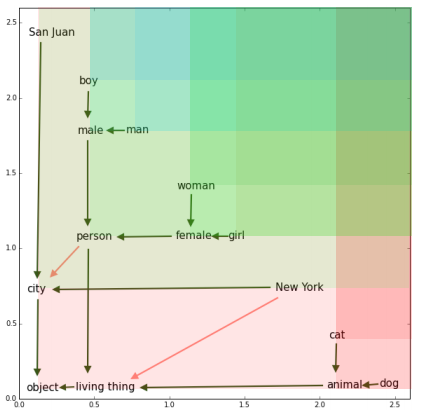
\includegraphics[width=.8\linewidth]{img/orderembboxed.png}  
          \caption{\textit{Order Embeddings}}
          \label{subfig:orderemb}
    \end{subfigure}
    \begin{subfigure}{.33\textwidth}
          \centering
          % include first image
          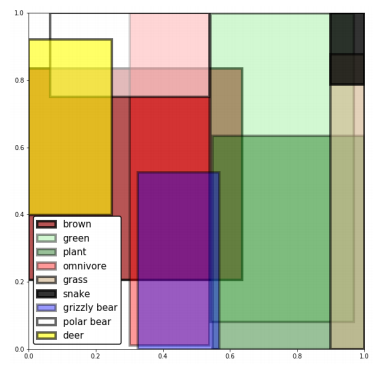
\includegraphics[width=.8\linewidth]{img/emb-boxlattice.png}  
          \caption{\textit{Box-Lattice Embeddings}}
          \label{subfig:boxlatticeemb}
    \end{subfigure}
    \begin{subfigure}{.33\textwidth}
          \centering
          % include first image
          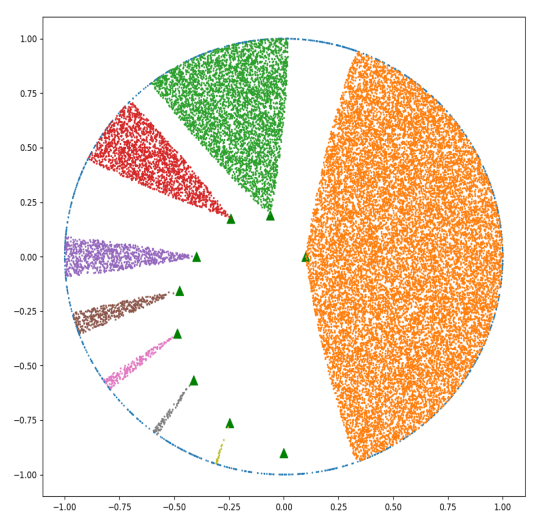
\includegraphics[width=.8\linewidth]{img/emb-poincone.png}  
          \caption{Plongements de Poincaré}
          \label{subfig:poincone}
    \end{subfigure}
    \caption[Plongements lexicaux spécifiques à l'hyperonymie]{Zones d'hyponymies pour  différents modèles de plongement lexical utilisés pour la détection d'hyperonymes. La zone d'hyponymie associée à un concept contient tous les hyponymes de ce concept. Les illustrations proviennent, de gauche à droite, de \cite{vendrov2015order}, \cite{vilnis2018probabilistic} et \cite{ganea2018hyperbolic}.}
    \label{fig:litt-emb-models}
\end{figure}


\subsubsection{Regroupement hiérarchique sur les plongements lexicaux}

Parmi les méthodes qui reposent sur des plongements lexicaux, on s'intéresse ici à celles qui réalisent un regroupement ou partitionnement des données (en anglais : \textit{clustering}).

Un algorithme de regroupement hiérarchique aboutit à la même structure d'arbre qu'une taxonomie : une fois que l'on dispose de représentations vectorielles pour les concepts à hiérarchiser, il est donc naturel d'appliquer un tel algorithme pour obtenir une taxonomie. Plusieurs méthodes ont été proposées dans ce sens. \cite{gupta2016domain} propose un partitionnement divisif de plongements lexicaux : on part de l'ensemble de tous les concepts, représentés par des plongements lexicaux génériques, et on y applique la méthode des $k$-moyennes. Le nombre de clusters $k$ est obtenu de manière non-supervisée, en combinant 
critère du coude (en anglais : \textit{elbow method}), statistique du \textit{gap} et examen de la \textit{silhouette} (voir \cite[p.~126--130]{everitt2011cluster} pour une discussion sur ces méthodes). Chaque cluster est alors étiquetté à l'aide d'une combinaison de motifs de Hearst, d'analyse statistique et de supervision humaine. Cette nouvelle étiquette est soit l'un des concepts contenus dans le cluster, soit un nouveau nom fourni par un annotateur humain. Puisque la méthode demande une supervision humaine, elle ne résout pas la question cruciale de l'étiquettage automatique des clusters, que nous examinons dans ce mémoire, dans les sections \ref{subsec:te-mapping} (cas non-expressif) et \ref{subsec:texp-exaxiom} (cas expressif). TaxoGen \cite{zhang2018taxogen} propose une méthode pour extraire une taxonomie à partir d'un regroupement hiérarchique de plongements vectoriels. TaxoGen repose sur un partitionnement adaptatif des données, capable de décider, pour chaque cluster, si une instance doit être propagée vers les sous-clusters (c'est-à-dire qu'elle peut être rattachée à un concept plus spécifique que le concept associé au cluster courant), ou si elle doit rester dans le cluster courant (ce qui signifie qu'elle n'est instance d'aucun concept plus spécifique). En revanche, TaxoGen ne propose pas de mécanisme pour associer un nom à chaque cluster : le résultat est donc une hiérarchie de groupes d'instances, et pas un ensemble d'axiomes de subsumption. À nouveau, la question de l'étiquettage automatique des clusters n'est pas résolue.
VDGEC \cite{zhang2018variational2} extrait de corpus textuels un graphe de co-occurrence de concepts, qui relie entre eux les concepts apparaissants fréquemment ensembles. Ce graphe est alors utilisé pour calculer des représentations vectorielles des concepts; ces vecteurs sont ensuite regroupés hiérarchiquement pour donner une taxonomie. La différence essentielle entre la méthode VDGEC et la nôtre est la nature des plongements vectoriels manipulés : dans VDGEC, on utilise directement les \textit{concepts}, alors que nous utilisons les \textit{instances}. Manipuler les instances ajoute une complexité supplémentaire, puisque les données à manipuler sont plus nombreuses, et qu'il est nécessaire de concevoir un mécanisme pour relier chaque concept à un groupe d'instances; en contrepartie, cela autorise une plus grande souplesse, particulièrement en permettant d'identifier de nouveaux groupes d'instances pertinents, et donc de nouveaux concepts. Nous démontrons cette possibilité dans le chapitre \ref{chap:texp}.

%\subsubsection{Extraction d'ontologies à partir de texte}
%Text2Onto, OntoCmaps, OntoGen
%Au-delà de l'extraction de taxonomies, plusieurs méthodes ont été proposées pour extraire directement des ontologies à partir de textes \cite{cimiano2005text2onto, zouaq2011towards, fortuna2007ontogen, haidar2016automatic}. Une approche fructueuse consiste à effectuer une analyse syntaxique des textes traités et à identifier des motifs à partir de l'arbre syntaxique obtenu. Ces motifs incluent les motifs de Hearst cités plus haut, qui servent à former des liens taxonomiques, mais ils sont étendus à d'autres types de relation. 
%La plupart de ces méthodes sont semi-automatiques \cite{cimiano2005text2onto, zouaq2011towards, fortuna2007ontogen}, c'est-à-dire qu'elles 


% \cite{petrucci2018expressive} propose d'appliquer les techniques développées pour la traduction automatique du langage naturel au problème de l'extraction d'axiomes : le but est de traduire une phrase en langage naturel vers la logique descriptive à l'aide d'un réseau de neurone récurrent. Par exemple, la phrase «une abeille est un insecte qui produit du miel» devrait être traduite en $\texttt{Abeille} \sqsubset \texttt{Insecte} \sqcap \exists \texttt{produit} . \texttt{Miel}$. Cette approche est toutefois limité par la rareté des données : il n'existe pas de corpus étendu établissant une correspondance entre langue naturelle et logique, ce qui conduit à des performances assez faibles.


intégrer les remarques ci dessous


\subsection{Extraction d'ontologies à partir d'un graphe}
\label{subsec:litt-te-graph}


% \hl{Bla bla extraction à partir de graphe}
% On présente d'abord les méthodes symboliques, qui utilisent les règles et le formalisme de la logique. Ces méthodes sont pour la plupart mal adaptées aux graphes de connaissances créés automatiquement ou semi-automatiquement, et ce pour deux raisons essentielles : d'une part, ces méthodes demandent beaucoup de ressources, et ne fonctionnent que sur des ontologies réduites; d'autre part, elles sont incapables de gérer correctement l'incertitude et le bruit qui caractérise ces graphes. 

Ici, on décrit les approches existantes pour extraire ou étendre une ontologie à partir d'un graphe de connaissance. % Là où les approches textuelles sont limitées à l'apprentissage de taxonomie, les méthodes basées sur les graphes permettent plus facilement d'extraire des axiomes expressifs. 
Par rapport à l'utilisation de corpus textuels, l'utilisation d'un graphe permet d'éviter les ambiguïtés syntaxiques ou lexicales, puisque l'on travaille directement à partir de données structurées.
On cherche généralement à exprimer les axiomes extraits dans le formalisme de la logique descriptive; certaines des méthodes présentées ici utilisent d'autres systèmes logiques (règles d'association, programme logique); sous réserve que ces systèmes sont moins expressifs que la logique descriptive $\mathcal{SROIQ}$, le passage de l'un à l'autre ne pose pas de problème.

Une première approche consiste à utiliser des techniques issues de l'intelligence artificielle symbolique pour effectuer des raisonnements à partir de règles existantes et déduire de nouveaux axiomes. D'autres méthodes identifient au contraire des régularités dans le graphe, soit par un examen statistique (fréquences relatives des relations et des concepts, calculs de co-occurrences), soit en plongeant les éléments du graphe dans une espace vectoriel qui reflète la structure du graphe. Ces différentes méthodes sont décrites dans les sections suivantes.


\subsubsection{Méthodes symboliques}

Les méthodes symboliques constituent une première famille d'approches capables de construire de nouveaux axiomes à partir d'axiomes existants. On désigne sous ce nom toutes les méthodes qui manipulent directement des règles logiques.
Ces méthodes sont pour la plupart mal adaptées aux graphes de connaissances créés automatiquement ou semi-automatiquement, et ce pour deux raisons essentielles : d'une part, ces méthodes demandent beaucoup de ressources, et ne fonctionnent que sur des ontologies réduites; d'autre part, elles sont incapables de gérer correctement l'incomplétude et le bruit qui caractérise ces graphes.  On en présente succintement trois grandes familles dans les paragraphes qui suivent.

Les \textbf{raisonneurs}, comme Fact++ \cite{tsarkov2006fact++} ou Hermit \cite{glimm2014hermit}, appliquent des règles de démonstration pour déduire des axiomes nouveaux. Un exemple de ces règles de démonstration est le \textit{modus ponens}, qui consiste simplement en $P \land (P \implies Q) \vdash Q$ : si $P$ est vraie et $P$ implique $Q$, alors $Q$ est vraie. Ces raisonneurs peuvent être utiles pour vérifier si une ontologie donnée est consistante, mais ils ne peuvent pas réellement être utilisés pour l'extraction de taxonomie : 
d'une part, ils nécessitent une ontologie de départ; d'autre part, ce sont des méthodes \textit{déductives} et donc incapables d'inférer de nouvelles règles à partir des données. %; enfin, la complexité de calcul augmente rapidement, ce qui les rend inadaptés pour des ontologies de grande taille.

Une autre approche symbolique \cite{cropper2020turning} est la \textbf{programmation logique inductive} (ou ILP, pour \textit{Inductive Logic Programming}) \cite{nienhuys1997foundations, de2008probabilistic}: il s'agit cette fois d'une méthode \textit{inductive}, c'est-à-dire qui produit de nouveaux axiomes à partir d'exemples. La programmation logique inductive part d'une série d'axiomes (la \textit{théorie préalable}, éventuellement vide) et d'exemples positifs et négatifs; elle cherche à produire de nouveaux axiomes qui sont vérifiés par les exemples positifs  mais pas par les exemples négatifs. De manière informelle et à titre d'exemple, on se donne une propriété $P$, une théorie préalable vide, un ensemble d'exemples positifs $E^+=\{P(0), P(2), P(4), P(8) \}$ et $E^- = \{ P(1), P(3), P(5) \}$ – autrement dit, $0, 2, 4, 8$ vérifient $P$ et $1, 3, 5$ ne la vérifient pas\footnote{Exemple tiré de \cite{nienhuys1997foundations}.}. Alors, un exemple de théorie induite est donné par :
\begin{align}
    & \textrm{Si } P(x) \textrm{ est vraie, alors } P(x + 2) \textrm{ est vraie.} \\
    & P(0) \textrm{ est vraie.}
\end{align}
Cette théorie ne pourrait être obtenue par un raisonneur, car elle n'est pas une conséquence logique de $E^+$ et de $E^-$ : il s'agit simplement d'une théorie plausible étant donné les faits observés. Pour obtenir des théories induites pertinentes, l'ILP nécessite donc un choix judicieux d'exemples positifs et négatifs.
Pour obtenir une théorie induite, 
on part d'une théorie initiale, possiblement vide, puis on l'améliore itérativement : si elle est trop générale, on la spécialise; si elle est trop spécifique, on la généralise \cite[p. 169]{nienhuys1997foundations}.
%deux approches sont possibles : soit partir d'une théorie très générale et la spécialiser itérativement en ajoutant des axiomes ou en précisant les axiomes existants, soit partir d'une théorie très spécifique et la généraliser itérativement.
En pratique, et comme pour les raisonneurs, les méthodes d'ILP passent difficilement à l'échelle pour les graphes de connaissance de grande taille \cite{srinivasan2012data}, même si des heuristiques moins coûteuses en calcul ont été proposées \cite{zeng2014quickfoil}. De plus, les données d'un graphe réel sont incomplètes et bruitées, une situation pas ou mal gérée par la programmation logique. 

Dans notre mémoire (section \ref{subsec:texp-exaxiom}), nous proposons une méthode d'extraction d'axiomes dont le point de départ est proche de l'ILP : on se donne en effet un ensemble d'exemples positifs et négatifs, et on cherche à trouver des axiomes décrivant l'un et pas l'autre. On résout le problème du passage à l'échelle en restreignant drastiquement l'espace de recherche grâce à l'utilisation de plongements vectoriels et du tirage aléatoire (\textit{sampling}). On reprend l'idée d'une amélioration itérative des axiomes par généralisation/spécialisation, mais on gère le bruit et l'incomplétude des données en utilisant des méthodes statistiques plutôt que symboliques.

Une troisième approche symbolique repose sur l'\textbf{analyse formelle de concept} (AFC, en anglais :  \textit{Formal Concept Analysis}), introduite mathématiquement par \cite{wille1982fca} et appliquée à la construction d'ontologie par \cite{cimiano2004conceptual}. L'AFC considère un ensemble d'entités possédant des attributs, et cherche à produire une hiérarchie de \textit{concepts} : dans ce contexte, un concept est une paire $(A, B)$ où $A$ est un ensemble d'entités et $B$ un ensemble d'attributs tels que $B$ est l'ensemble des attributs vérifiés par tous les éléments de $A$, et inversement $A$ est l'ensemble des entités qui vérifient tous les attributs de $B$. L'ensemble des concepts est muni d'une relation d'ordre $\sqsubseteq$ : on a $(A, B) \sqsubseteq (A', B')$ si $A \subseteq A'$ (ou, de manière équivalente, $B' \subseteq B$), analogue à la subsumption décrite plus haut. Munie de cette relation d'ordre, l'AFC induit naturellement une hiérarchie sur les concepts : l'enjeu est donc de construire une série de concepts pertinents.
Pour obtenir ces concepts, on utilise une règle de dérivation : si $A$ est un ensemble d'entités, on désigne par $A'$ l'ensemble des attributs communs à tous les éléments de $A$; de la même manière, si $B$ est un ensemble d'attributs, on désigne par $B'$ l'ensemble des entités qui possèdent tous les attributs de $B$. En partant d'une entité $x$, on peut ainsi obtenir $\{x\}'$ l'ensemble des attributs de $x$, puis $\{x\}''$ l'ensemble des entités qui ont exactement les mêmes attributs que $x$ : la paire $(\{x\}'', \{x\}' )$ constitue un premier concept. En ajoutant une nouvelle entité $y$ à $\{x\}''$, on obtient un nouvel ensemble d'entités $\{x \}'' \cup \{ y\}$, que l'on peut à nouveau dériver en un ensemble d'attributs  $(\{x \}'' \cup \{ y\})'$, lui-même dérivé pour former un second concept $((\{x \}'' \cup \{ y\})'', (\{x \}'' \cup \{ y\})'\}$; et ainsi de suite. Par ailleurs, un ensemble de concepts $C_1, \ldots, C_N$ possède toujours un \textit{sous-concept commun maximal}, c'est-à-dire le plus grand concept $S$ qui vérifie $\forall i, S \sqsubseteq C_i$. De même, chaque ensemble de concepts possède un \textit{superconcept commun minimal}, c'est-à-dire le plus petit concept $S$ tel que $\forall i, C_i \sqsubseteq S$. De plus, il existe un concept minimal, qui contient tous les attributs (et potentiellement aucune entité), et un concept maximal, qui contient toutes les entités (et potentiellement aucun attribut). 
%Le formalisme de l'AFC possède des soubassements mathématiques bien étudiés, mais la conception d'algorithmes efficaces et appropriés à des graphes de grande taille demeure un problème ouvert
À partir de ces notions, de nombreux algorithmes ont été proposés pour l'identification et la hiérarchisation de concepts \cite{valtchev2001building, nourine1999fast, farach2008linear}; 
toutefois, la conception d'algorithmes efficaces et applicables à grande échelle demeure un problème ouvert %ce problème continue à faire l'objet de recherches actives, notamment pour en réduire la complexité et donc permettre des applications à des jeux de données étendus 
\cite{li2016approximate, zhang2019new}.
L'AFC peut être étendue aux relations binaires, c'est-à-dire à des triplets $(h, r, t)$ où $h, t$ sont des entités reliées par la relation $r$ : on parle alors d'\textbf{analyse relationnelle de concept} (ARC, ou \textit{Relational Concept Analysis} en anglais) \cite{bendaoud2008rcafca}. % Une autre extension de l'AFC consiste à remplacer la logique booléenne usuelle par la logique floue, qui accepte des valeurs de vérité continues entre 0 et 1 et qui permet de mieux modéliser l'incertitude \cite{de2012hierarchical, mao2019construction}.

\subsubsection{Méthodes statistiques}

Les méthodes statistiques visent à extraire des règles logiques en observant des régularités statistiques dans un graphe de connaissance : par exemple, en comptant les co-occurrences de certaines classes ou de certaines relations dans le voisinage d'une entité. 

On présente ici la méthode de \textit{Statistical Schema Induction} (SSI, en français : induction statistique d'ontologie) \cite{volker2011statistical}, qui se rapproche du travail que nous présentons à la section \ref{subsec:texp-exaxiom}. Cette approche repose sur l'apprentissage de \textit{règles d'association} \cite{zhang2003association}, qui sont essentiellement des implications logiques inférées d'après des co-occurrences observées dans les données. 
Une règle d'association s'écrit sous la forme $X \rightarrow Y$. On peut par exemple imaginer une règle $\{\texttt{Personne}, \exists \texttt{écrit}.\texttt{Poème} \} \rightarrow \texttt{Poet}$ : si une même entité est de type \texttt{Personne} et vérifie l'axiome $\exists \texttt{écrit}.\texttt{Poème}$, alors cette entité est probablement de type \texttt{Poète}.

Pour extraire ces règles, on se donne un \textit{tableau de transactions} $\textbf{T}$, c'est-à-dire une matrice dont les lignes représentent les entités $e_1, \ldots, e_n$ du graphe, et les colonnes des prédicats logiques $P_1, \ldots, P_m$. Ces prédicats incluent les concepts nommés $C$ (comme \texttt{Artist}, \texttt{Person}, etc.) et différentes formes de restrictions existentielles comme $\exists r.C$ ou  $\exists r.\top$. On note $\Ent$ l'ensemble des entités, et $\mathcal{P}$ l'ensemble des prédicats. 
La coordonnée $(i, j)$ de $\textbf{T}$ contient $1$ si $e_i$ vérifie le prédicat $P_j$, et $0$ sinon. Soit $X \subseteq \mathcal{P}$ un ensemble de prédicats, alors le \textit{support} de X est l'ensemble des entités qui vérifient tous ces prédicats simultanément :
\begin{equation}
    \textrm{Supp}(X) = \frac{|\{ e \in \Ent : \forall P \in X, P(e) \}|}{|\Ent |}
\end{equation}
L'indice de confiance associée à une règle $X \rightarrow Y$ se calcule alors par :
\begin{equation}
    \textrm{Conf}(X \rightarrow Y) = \frac{\textrm{Supp}(X \cup Y)}{\textrm{Supp}(X)}
\end{equation}
Au numérateur, on compte le nombre d'entités qui vérifient à la fois les prédicats de $X$ et de $Y$, que l'on rapporte au nombre d'entités qui vérifient les prédicats de $X$ (notons que l'on a nécessairement $\textrm{Supp}(X \cup Y) < \textrm{Supp}(X)$, car une entité qui vérifie à la fois les prédicats de $X$ et de $Y$ vérifie \textit{a fortiori} ceux de $Y$). Un indice égal à $1$ signifie que toutes les entités qui vérifient $X$ vérifient également $Y$, et donc que la règle $X \rightarrow Y$ est parfaitement validée par les données; dans la pratique, on définit plutôt un seuil $\tau$ au-delà duquel la règle d'association est considérée comme valide.

Le nombre de combinaisons de prédicats possibles croît exponentiellement : les énumérer est donc impossible, même pour des jeux de données réduits. Plusieurs heuristiques ont été développées, dont la plus connue est Apriori \cite{srikant1994apriori}, elle-même améliorée à plusieurs reprises, par exemple en minimisant le nombre de lectures du graphe \cite{yuan2017improved} ou en implémentant un mécanisme de parallélisme avec MapReduce \cite{lin2014mapreduce}. % Autres approches : FP-growth, OPUS

Une fois les règles d'association extraites, on peut les filtrer et les convertir en axiomes de subsumption. Cette approche produit des axiomes de subsumption isolés les uns des autres, alors qu'on souhaite généralement obtenir une hiérarchie contenant tous les concepts nommés et, éventuellement, de nouveaux concepts expressifs. Dans notre propre méthode, nous reprenons l'idée d'extraire des axiomes en examinant statistiquement un tableau de co-occurrence entités-axiomes. Notre méthode propose toutefois deux différences essentielles : d'une part, elle s'applique sur un groupe d'entités restreint, qui a été défini de manière non supervisée en se basant sur des plongements vectoriels; d'autre part, l'extraction d'axiomes sert uniquement à \textit{étiquetter} des groupes d'entités, et non pas à obtenir des liens de subsumption. Dans notre cas, les relations de subsumptions sont identifiées par regroupement hiérarchique.



% À partir de textes
% Traduction d'axiomes depuis le langage naturel
\subsubsection{Utilisation de plongements vectoriels de graphe pour l'extraction d'ontologies}

Un modèle de plongement vectoriel de graphe est un modèle capable de construire des représentations vectorielles des entités et des relations d'un graphe de connaissance. Il s'agit d'une approche relativement récente qui présente une analogie forte avec les plongements lexicaux utilisés en traitement de la langue. Les modèles de plongement constituent un aspect important de notre travail, et sont décrits en détail dans le chapitre \ref{chap:kge} – on renvoie donc le lecteur à ce chapitre pour une plus ample présentation. Dans cette section, il suffit de savoir qu'un modèle de plongement associe à chaque entité $e$ du graphe un vecteur $\textbf{e} \in \R^d$ (plus rarement $\mathbb{C}^d$), de telle sorte que deux entités impliquées dans des relations similaires aient des plongements géométriquement proches.

Les plongements vectoriels de graphes de connaissance sont très utilisés pour découvrir des régularités au niveau des instances (ce qui permet notamment d'évaluer la validité d'un triplet inconnu ou de prédire de nouveaux triplets), mais ils ont encore été peu exploités pour la manipulation de concepts ou l'extraction de taxonomie ou d'ontologie. Dans cette optique, \cite{gutierrez2018knowledge} étudie les liens entre les axiomes logiques et la géométrie de différents modèles de plongement, dans le but de pouvoir traduire un axiome sous forme de plongement vectoriel sans perte d'information ou d'expressivité. Une idée qui commence à se développer consiste à utiliser les plongements vectoriels pour évaluer \textit{a priori} la plausibilité d'un axiome logique, ce qui permet de réduire l'espace de recherche. Dans cette lignée, IterE \cite{zhang2019iteratively} apprend conjointement des plongements vectoriels et des règles logiques, les deux se renforçant mutuellement. Des plongements sont initialement appris à partir du graphe de connaissance; ensuite, une marche aléatoire dans le graphe permet de générer des axiomes potentiels. Ces axiomes se voient alors attribuer un score de vraisemblance, grâce à une table de correspondance entre axiomes logiques et plongements. Par exemple, l'axiome $A \equiv B$ est traduit géométriquement par $\textbf{A} = \textbf{B}$, où $\textbf{A}$ et $\textbf{B}$ sont les plongements vectoriels des concepts $A$ et $B$. Le score de vraisemblance de $A \equiv B$ est alors défini comme la similarité géométrique des plongements de $A$ et de $B$ : dans le cas idéal où $\textbf{A} = \textbf{B}$, la similarité est maximale et l'axiome obtient un score de 1. Plus on s'éloigne de ce cas idéal, plus le score diminue. Cette approche permet une évaluation peu coûteuse des axiomes candidats. Enfin, les axiomes ayant un score de vraisemblance suffisamment haut servent à générer de nouveaux triplets d'entraînement : on peut alors répéter ces trois étapes pour améliorer itérativement les plongements et les axiomes. Cette méthode est uniquement évaluée sur des graphes de petite taille (moins de 50 000 entités); savoir si elle est applicable à plus large échelle reste une question ouverte. RLvLR \cite{omran2018scalable} repose sur un principe similaire. Il cherche à extraire des règles logiques de la forme $x \overset{r_1}{\longrightarrow} z_1 \overset{r_2}{\longrightarrow} z_2  \overset{r_3}{\longrightarrow} \ldots  \overset{r_k}{\longrightarrow} y$ $\implies \rel{x}{r}{y}$. entre les relations. Pour une relation $r$ donnée, on récupère les triplets impliquant $r$, puis on effectue des marches aléatoires autour de ces triplets pour générer des règles candidates. Ces règles sont alors filtrées en exploitant la similarité des plongements des relations impliquées dans chaque règle. Cela permet de restreindre l'espace de recherche et donc d'appliquer la méthode à des graphes de grande taille comme Wikidata ou DBpedia. En contrepartie, l'expressivité des axiomes extraits est limitée; de plus, les axiomes extraits ne sont pas organisés entre eux sous forme de taxonomie.


\phantomsection
\label{subsec:litt-tiemb}


Plus proche de notre propre méthode, \textbf{TIEmb} \cite{ristoski2017large} extrait une taxonomie (non-expressive) à partir de plongements vectoriels d'entités. Comme notre méthode, TIEmb considère comme données d'entrée un ensemble de paires $\{(\textbf{e}_i, t_i) \}_{i=1, \ldots, n}$, où $\textbf{e}_i \in \R^d$ est le plongement vectoriel de l'entité $e_i$, et $t_i$ est son type, et produit en sortie une taxonomie, c'est-à-dire un ensemble d'axiomes de subsumption de la forme $t_i \sqsubset t_j$. Pour cela, chaque type $t$ est représenté par un sphère $S_t$ à $d$ dimensions, dont le centre est un vecteur $\textbf{c}_t$ défini par :
\begin{equation}
 \textbf{c}_t = \frac{1}{n_t} \sum_{\substack{i \in [1, n] \\ t_i = t}} \textbf{e}_i
\end{equation}
Avec $n_t = |\{ i \in [1, n] : t_i = t \}|$ le nombre d'entités de type $t$ dans les données. $\textbf{c}_t$ représente le centroïde des instances de $t$.

Le rayon $r_t$ de $S_t$ est lui défini comme la distance moyenne entre les instances de $t$ et le centroïde $\textbf{c}_t$ :
\begin{equation}
    r_t = \frac{1}{n_t}  \sum_{\substack{i \in [1, n] \\ t_i = t}} \| \textbf{e}_i - \textbf{c}_t \|_2
\end{equation}


\begin{figure}[h]
    \centering
    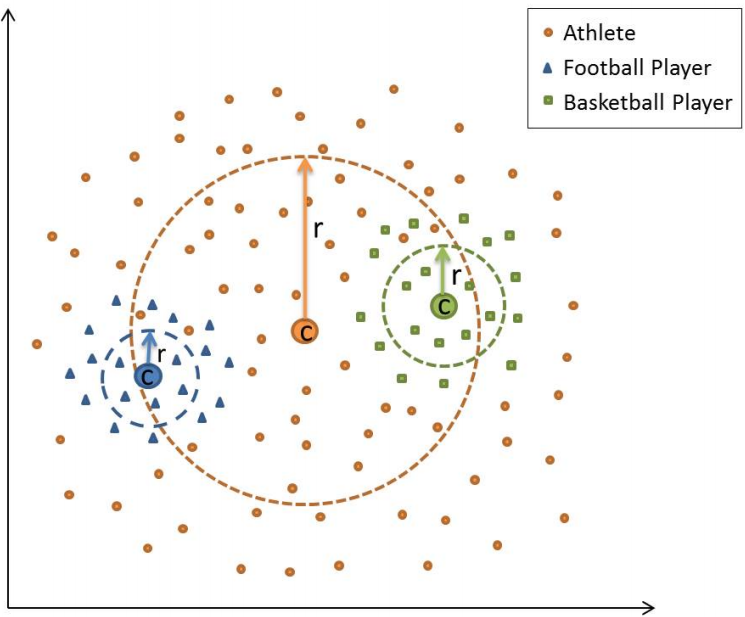
\includegraphics[width=0.5\textwidth]{img/tiemb.png}
    \caption[Principe général de TIEmb]{Plongements et sphères associées à trois classes dans le cadre de la méthode TIEmb, dans le cas bidimensionnel. Illustration tirée de \cite{ristoski2017large}.}
    \label{fig:litt-tiemb}
\end{figure}


Dès lors, l'axiome $t \sqsubset t'$ est prédit si et seulement si $S_t \subset S_{t'}$ : la sphère d'un supertype englobe les sphères de ses sous-types, comme illustré à la figure \ref{fig:litt-tiemb}. Enfin, une étape finale de filtrage est appliquée pour enlever les cycles et obtenir une taxonomie valide. 

TIEmb présente l'avantage d'être conceptuellement simple, et peu coûteux en calcul, ce qui permet de l'appliquer à très grande échelle. Une différence cruciale avec notre approche est que le regroupement des entités au sein des sphères est entièrement supervisé, puisqu'il repose sur les types $t_i$ contenus dans les données, et pas sur la géométrie des plongements : TIEmb ne permet donc pas d'identifier de nouveaux groupes cohérents d'entités et donc de détecter de nouvelles classes. Dans le chapitre \ref{chap:te}, on compare notre méthode d'extraction de taxonomie non-expressive à TIEmb; dans le chapitre \ref{chap:texp}, on illustre les possibilités offertes par le regroupement non-supervisé en extrayant une taxonomie expressive de DBpedia.

\paragraph{Résumé}

On a présenté un aperçu de différentes approches pour extraire automatiquement des taxonomies ou des ontologies. Parmi ces méthodes, celles qui manipulent directement un graphe ou des textes se heurtent à deux difficultés : d'une part, les données sont \textit{sparse} (parfoit traduit par «disséminées» ou «creuses» en français), c'est-à-dire que de nombreux éléments (mots ou entités) sont rarement observés; d'autre part, les données sont \textit{discrètes}, et généraliser les observations faites sur un élément à d'autres éléments est compliqué.

Les plongements vectoriels permettent de surmonter ces deux difficultés, et ont été appliquées à l'extraction d'ontologies avec une grande variété de méthodes et d'objectifs.
Toutefois, aucune des méthodes présentées ne permet d'extraire une ontologie complète et de haute qualité sans supervision humaine. %Le problème demeure donc ouvert. 
Les modèles capables d'induction complexe ne sont généralement pas applicables sur des graphes de grande taille comme DBpedia. À l'inverse, les modèles capables de passer à l'échelle se contentent de hiérarchiser des classes existantes, et sont incapables d'identifier de nouvelles classes à partir des données. 
Dans la suite, nous proposons une méthode capable d'extraire une taxonomie expressive à grande échelle, en combinant plongements vectoriels de graphe, regroupement hiérarchique non-supervisé et extraction d'axiome à partir de statistiques sur le graphe.